\pdfminorversion=4
\documentclass[hidelinks]{report}

\usepackage{graphicx}
\usepackage{times}
\usepackage{plain}
\usepackage[plainpages=false]{hyperref}
\usepackage{courier}
\usepackage{caption}

% To force figures to appear after text(along with [H] option)
\usepackage{float}

% To apply linespacing to some content
\usepackage{setspace}

% To show commands, code snippets
\usepackage{listings}

% To use checkmark (tick symbol)
\usepackage{amssymb}

\graphicspath{ {images/pdf/} }

\pagestyle{plain}

\fontfamily{Times}
\selectfont

\setlength{\textwidth}{6.5in}
\setlength{\textheight}{8.5in}
\setlength{\topmargin}{-0.25in}
\setlength{\oddsidemargin}{-0.00in}
\setlength{\evensidemargin}{-0.00in}

% To use multirow feature of latex tables
\usepackage{multirow}

% Using and defining own color
\usepackage{color}
\definecolor{mycol}{RGB}{52, 43, 41}

% Defining courier font usage syntax
\newcommand{\cf}[1] {
	\textbf{\texttt{#1}}
}

% Defining checkmark usage syntax
\newcommand{\T} {
	\checkmark
}

\begin{document}

%% Line spacing 1.5 applied
\setstretch{1.5}

\begin{center}
\section*{vEPC 1.0 Developer Manual}
\end{center}
We describe here the distributed architecture of vEPC 1.1 and discuss the strategies used to achieve them.\\

\paragraph*{NOTE:}

 Please go through Developer manual in vEPC 1.0 to know about 1) Design and implementation details of various software modules that were developed as part of our vEPC.2) A high level description of individual source code files (\cf{.cpp/.h}). Please read the \cf{user\_manual.pdf} under \cf{doc} folder for instructions on experimenting with our vEPC.


\begin{center}

\subsection*{ Design of a distributed vEPC}

\end{center}

We have designed and implemented various EPC modules (MME, HSS, SGW, PGW) along with a RAN simulator and a Sink node in vEPC 1.0 release. In current version we implemented a scalable design to the previous release. Now we describe the design of our distributed architecture which supports horizontal scaling.



%\begin{center}
\begin{figure}[H]
\centering
\frame{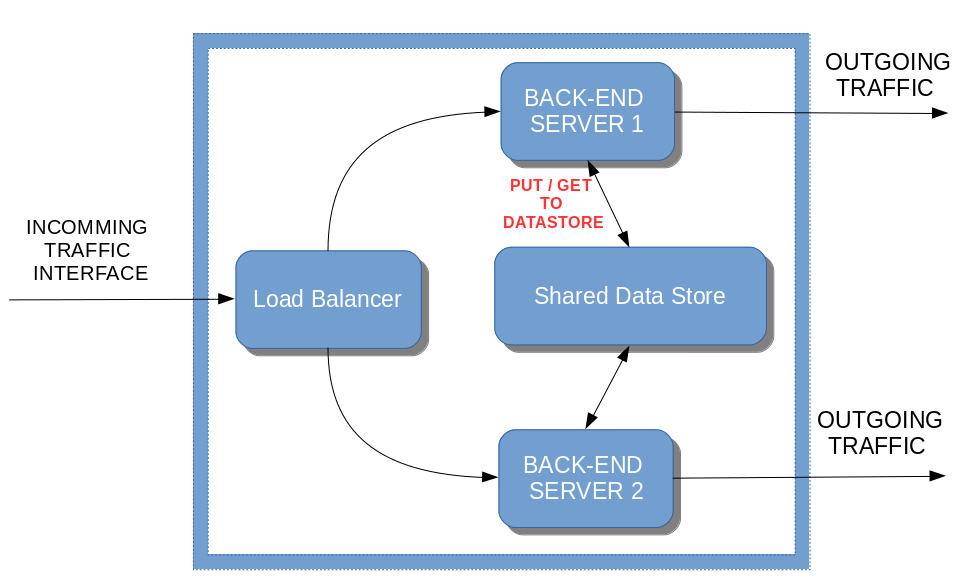
\includegraphics[scale=0.25]{single}}
\caption{Distributed architecture of single epc component
MME / SGW / PGW}
\label{fig:singlel}
\end{figure}
To transform the monolithic design to a scalable design, we need to replace the monolithic EPC components with a distributed  version of the same. Figure \ref{fig:singlel} shows a clustered version of an EPC element. In this design, architecture components namely MME, SGW and PGW are replaced by clusters consisting of a load balancer (LB), a shared data store (DS) and a number of back-end worker servers. 

\begin{center}
\begin{figure}[H]
\centering
\frame{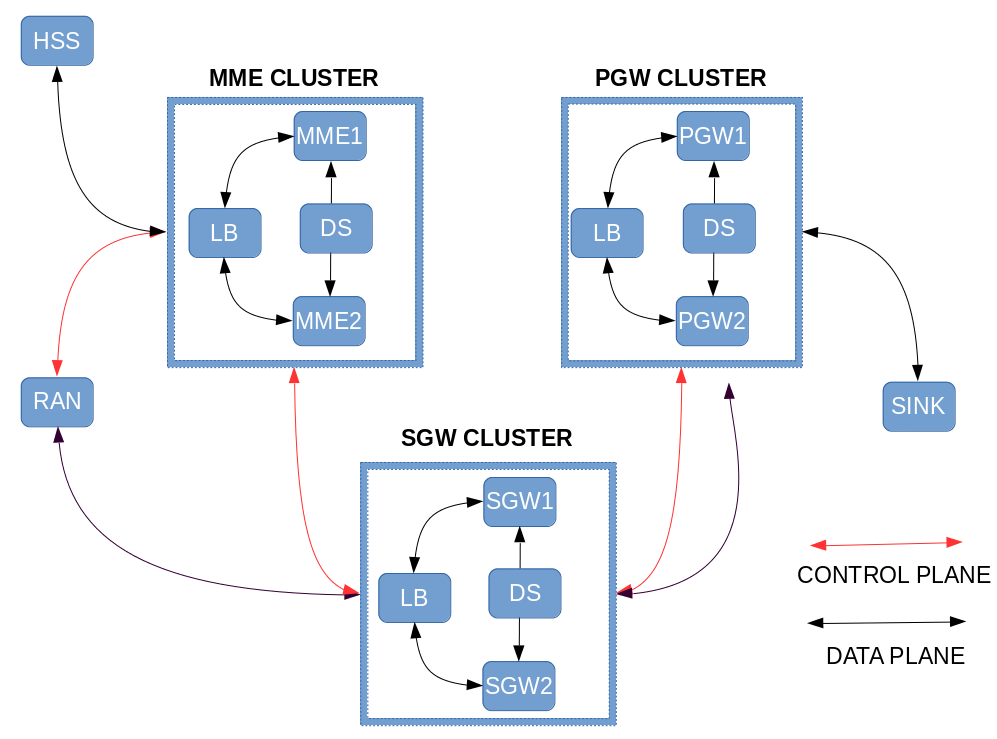
\includegraphics[scale=0.3]{overview}}
\caption{The complete distributed LTE EPC architecture for a two worker system}
\label{fig:overall}
\end{figure}
\end{center}
Overall architecture of the scalable EPC with distributed clusters in place of monolithic components is shown in Figure \ref{fig:overall}. Control-plane path has been highlighted in red and data-plane in black. This shows how each cluster interfaces with other components of the EPC system.

As shown in Figure \ref{fig:overall} each cluster (MME/SGW/PGW) contains a load-balancer as a front end element which acts as an interface to the other EPC components. The primary purpose of the load-balancer is to distribute incoming traffic to the worker nodes. In a single LTE procedures there are many request/response pairs. We call these request/response pairs as sub procedures. The LTE EPC protocol implementation requires that the sub procedure of a particular procedure e.g Attach should have access to the previously stored states. One way to achieve this is by synchronizing each sub-procedure state to the data store. As this approach has performance trade-off, we chose the design in which all sub procedures of a particular procedure e.g Attach are directed to a particular back-end server in the cluster. 

\begin{center}
\subsection*{Implementation}

\end{center}
Here we discuss implementation details of each of the component that was used to achieve a scalable design.
\subsection*{Load balancing:}
\label{lb}
We discuss about how load balancing was done at each of the clusters i.e MME cluster, SGW cluster and PGW cluster.

\subsubsection{\textbf{MME cluster load balancing:}}
MME load balancing consists balancing only control traffic.

For MME workers to be stateless we have to ensure that the local state gets pushed to the data store at the end of the session. In our implementation we classify the sequence of all sub-procedures of an attach request to be in one session. Similarly, we classify the Detach procedure to be in one session. With these session definitions we could afford to push state data to the data store only when that session ends. The above notion can only work when the sub-procedure of a procedure e.g. Attach are made to hit always the same worker till the procedure ends for a particular UE. As the sub-procedures in Attach are known to be on the same SCTP connection, We could configure the load-balancer to work in a round robin fashion for each new connection. Any packet that is part of an existing connection will get directed to the same MME worker. The LVS load balancer uses a hash of 5-tuple to keep track of established SCTP connection and their destination worker. With the implementation of this strategy we have to synchronize data with datastore only when the Attach procedure ends or the Detach procedure ends. When a UE performs attach successfully, it can perform detach even if the worker which performed the attach is no longer online. The load balancer can direct the request to one of the online workers. The detach request can easily be processed by another MME worker by extracting the store saved at the shared key-value store.


\subsubsection{\textbf{SGW cluster load balancing}}
SGW load balancing consists of two types of traffic (1) Control traffic (2) Data traffic

\textbf{Load-balancing control traffic:}

For SGW worker to be stateless, we have to push SGW worker states to the data store. The LTE Attach procedure has 2 sub procedures at SGW. Therefore, at end of each sub-procedure we have to push the state to datastore. We can reduce the number of state synchronization if we ensure that each of the sub-procedure for a particular UE lands up in the same SGW worker node. UDP based round robin load balancing in LVS can be configured to maintain UDP sessions (4 tuples of UDP connection). Using this we ensure that request from a particular UDP client always follows the same path. At MME we assign sub procedures of attach request of a particular UE to a particular UDP socket. We can group requests from a particular UE by hashing on IMSI of that UE. Hence all message in the same UDP session hit the same SGW replica. With this we need to synchronize the state at the end of the two sub procedure (the complete attach operation).

\par However, when the worker of SGW cluster fails after processing only one of the sub procedure, the intermediate state is lost and the procedure has to be re-initialized.\\

\textbf{Load-balancing data traffic:}

SGW is responsible for forwarding data packets from UE based on tunnel ids setup in the control plane. These tunnel ids are saved in the shared data store of SGW cluster. If each packet is sent with round robin approach to different workers then SGW worker has to extract the saved state of each such packet. To counter this trade-off we use the same concept of UDP session. When for a sequence of packets, the 4 tuple of UDP connection remains same, we call it a single UDP session. We  enforce the LVS UDP based Round robin load balancer to route data packets from a particular UE to the same SGW worker. Now we can keep a cache of the shared data store key values until the end of that UDP session. In this way we do not have to extract state each time a packet arrives. We ensure that for a data session the UDP 4 tuple between eNodeB and SGW remains the same. We use hash of the tunneled ip address of the packet to assign it to the same UDP client every time keeping the source address same. The destination address is always the SGW cluster load balancer. In this way for a particular UE we could ensure that UDP 4-tuple remains same. The UDP load-balancer hence directs packets of same UE to a particular SGW worker.

\par The same implementation was used when downlink traffic comes from PWG worker to SGW load balancers.
\begin{figure}[H]
\centering
\frame{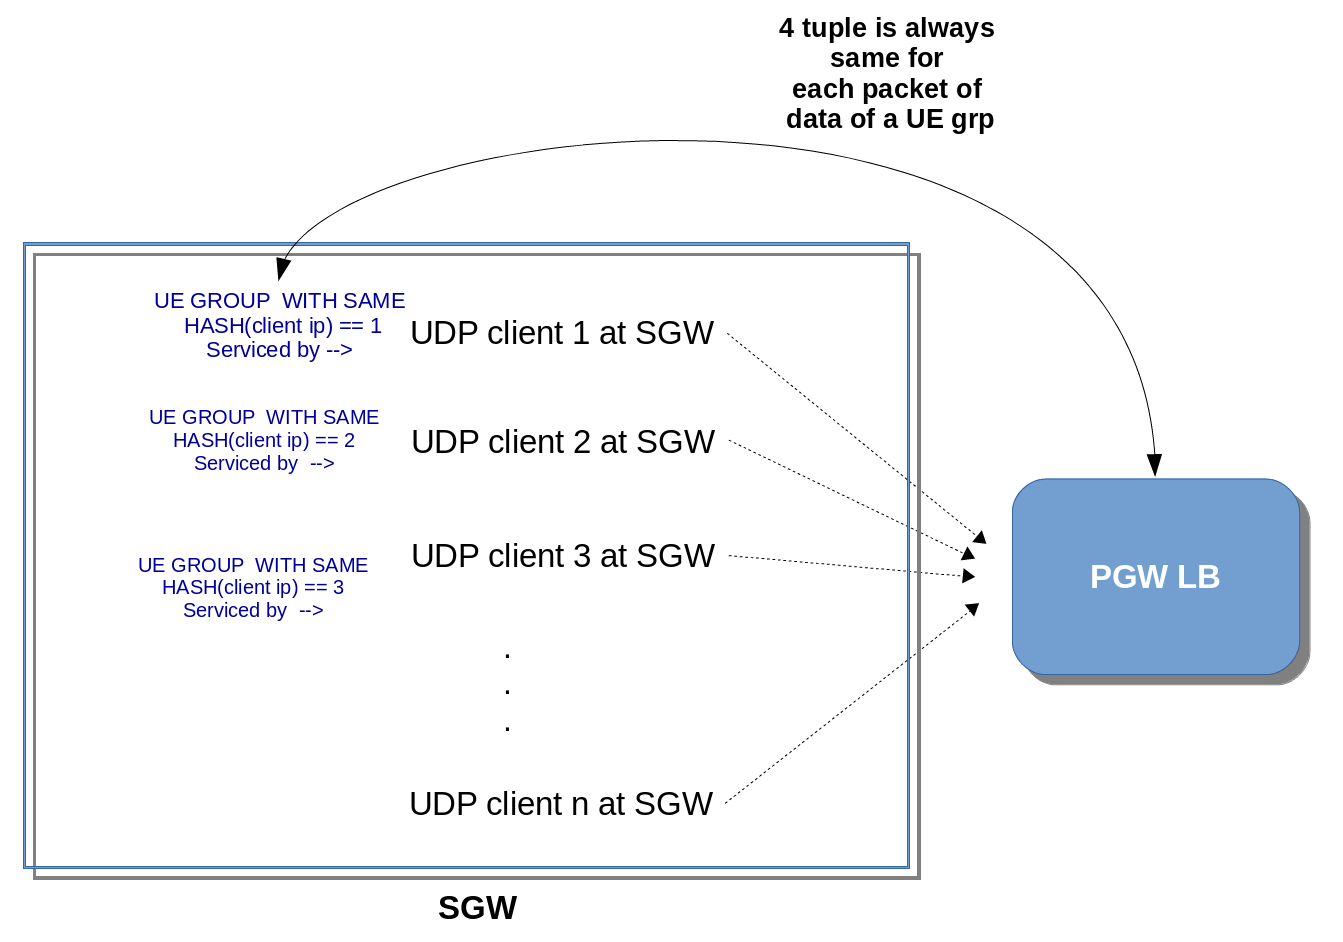
\includegraphics[scale=0.19]{sgwip}}
\caption{UE assignment to fixed udp clients at SGW}
\label{fig:sgwudp}
\end{figure}
\subsubsection{\textbf{PGW cluster loadbalancing}}
PGW load balancing consists of two types of traffic (1) Control traffic (2) Data traffic \\

\textbf{Load-balancing control traffic:}
Attach operation at PGW consists of only one sub-procedure. For PGW worker to be stateless, we push the saved state to data store at the end of the Attach procedure. 

\par When the worker of PGW cluster fails after processing Attach procedure, another worker can continue to process the other LTE procedures such as a Detach request by extracting the last saved state from data store.\\

\textbf{Load-balancing data traffic:}
%\begin{center}

PGW is responsible for forwarding data packets of UEs based on tunnel ids setup in the control plane. These tunnel ids are saved in the shared data store of PGW cluster. If each packet is sent with a round-robin approach then SGW worker has to extract the saved state of each such packet. To counter this trade-off we used the same strategy that was explained for SGW. Data traffic from a particular traffic can now be enforced to reach a particular PGW worker in a single UDP session by keeping the 4 tuple between SGW worker and PGW load balancer same. Figure \ref{fig:sgwudp} illustrates this idea. The UDP load-balancer hence directs packets of same UE to a particular PGW. By keeping the information in the cache of the worker we do not have to retrieve state from data store each time a packet arrives.
%\begin{center}

\par Same implementation has been followed for downlink traffic from sink to PGW load balancers. In this way we ensure that a particular UE's every data packet travels through the same back-end servers to reach sink. Figure \ref{fig:dpath} shows a possible flow of packets of three UE groups.
\begin{figure}[H]
\centering
\frame{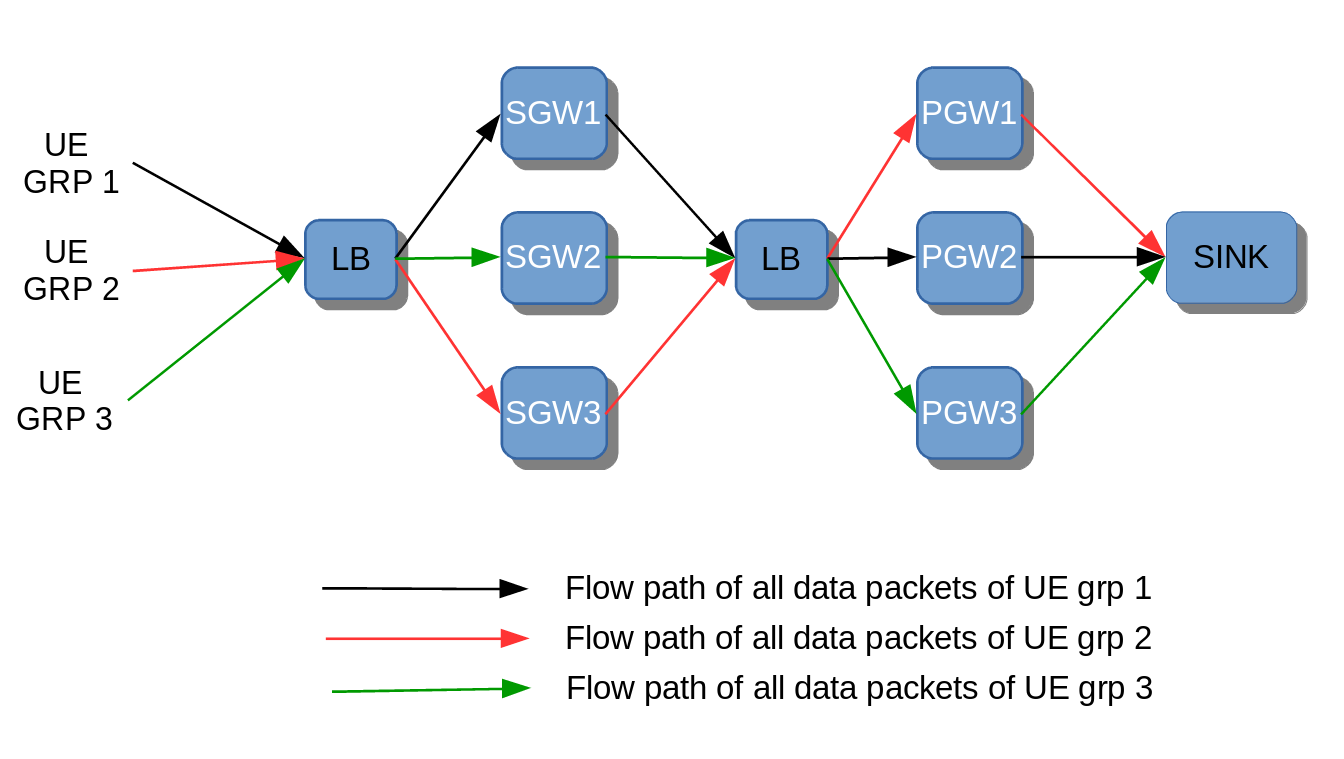
\includegraphics[scale=0.30]{dpath}}
\caption{UE data packet flow illustration}
\label{fig:dpath}
\end{figure}

\subsection*{Data store interfacing:}

As discussed in earlier sections MME cluster, SGW cluster and PGW cluster should have stateless workers in order to scale horizontally. This requires a shared data store (key-value store) in each of these clusters. As discussed in section \ref{lb} state synchronization is done at the end of an LTE procedure in MME, SGW and PGW workers.

\par In control plane operation of LTE EPC the saved states are pushed periodically to the shared datastore. This enables any back-end workers in the cluster to service a particular UE. As an example: a UE performs an Attach procedure which was serviced by MME worker1. When UE tries a Detach operation, any of the back-end workers can pull the saved states for that UE from the data store and proceed to perform Detach.
\par In data plane operation the UE context information is safely present in the shared datastore. When a UE sends data packets to SGW worker, the worker can pull the UE context from shared data store and perform packet forwarding.

\par The NFV-LTE-EPC 2.0 system was integrated to key value data stores using a library API present in src/client directory that provides interfacing to various key value stores.

\end{document}